\documentclass[twocolumn]{memoir}
\usepackage[british]{babel}


\usepackage{libertine}
\renewcommand*\familydefault{\sfdefault}  %% Only if the base font of the document is to be sans serif
% \usepackage[T1]{fontenc}
\usepackage{tabularx}
\usepackage{graphicx}

% \usepackage[utf8]{inputenc}
%\usepackage{flushend}
\usepackage{tcolorbox}

\usepackage{ragged2e}
\usepackage{microtype}
\usepackage{hyperref}

\setlength{\RaggedRightParindent}{\parindent}

\newtcolorbox{commentbox}{colback=red!5!white,colframe=red!75!black,title=Comment}
\newtcolorbox{tldr}{colback=blue!5!white,colframe=blue!75!black,title={TL;DR}}
\newtcolorbox{gmtip}{colback=blue!5!white,colframe=blue!75!black,title={GM tip!}}


\newenvironment{firstperson}{%
% \itshape%
% \fancybreak{\rule{0.7\linewidth}{1pt}}%
}{%
% \fancybreak{\rule{0.7\linewidth}{1pt}}%
}

\title{Giants of Cheddar Gorge}
\author{Nathanael Farley}


\begin{document}
\RaggedRight
\maketitle

\section{Introduction}
\begin{firstperson}
It is said that the inhabitants of Cheddar Gorge in 1566 have always been unusually tall. Some say they even descended from the Elorai, the ancient Giants of the Gorge. 

Of course, such things are a myth. At least, they were thought to be \ldots
\end{firstperson}

This adventure takes the players into the world of Cheddar Gorge as it might have been in 1566 had magic existed. 

\begin{commentbox}
More information about this magical Cheddar Gorge should be included here
\end{commentbox}

A darkness has struck the village in the form of a plague. There is an old story from many years ago of a similar plague that was cured by the Elorai, the supernatural Guardians of the Gorge. Since they are long gone, the only thing that remains of them is rumours of a labyrinth that contains the cure. Protected by traps, curses and monsters to prevent all but the most worthy to enter the sacred chamber and attain the cure.

\begin{figure}
\centering
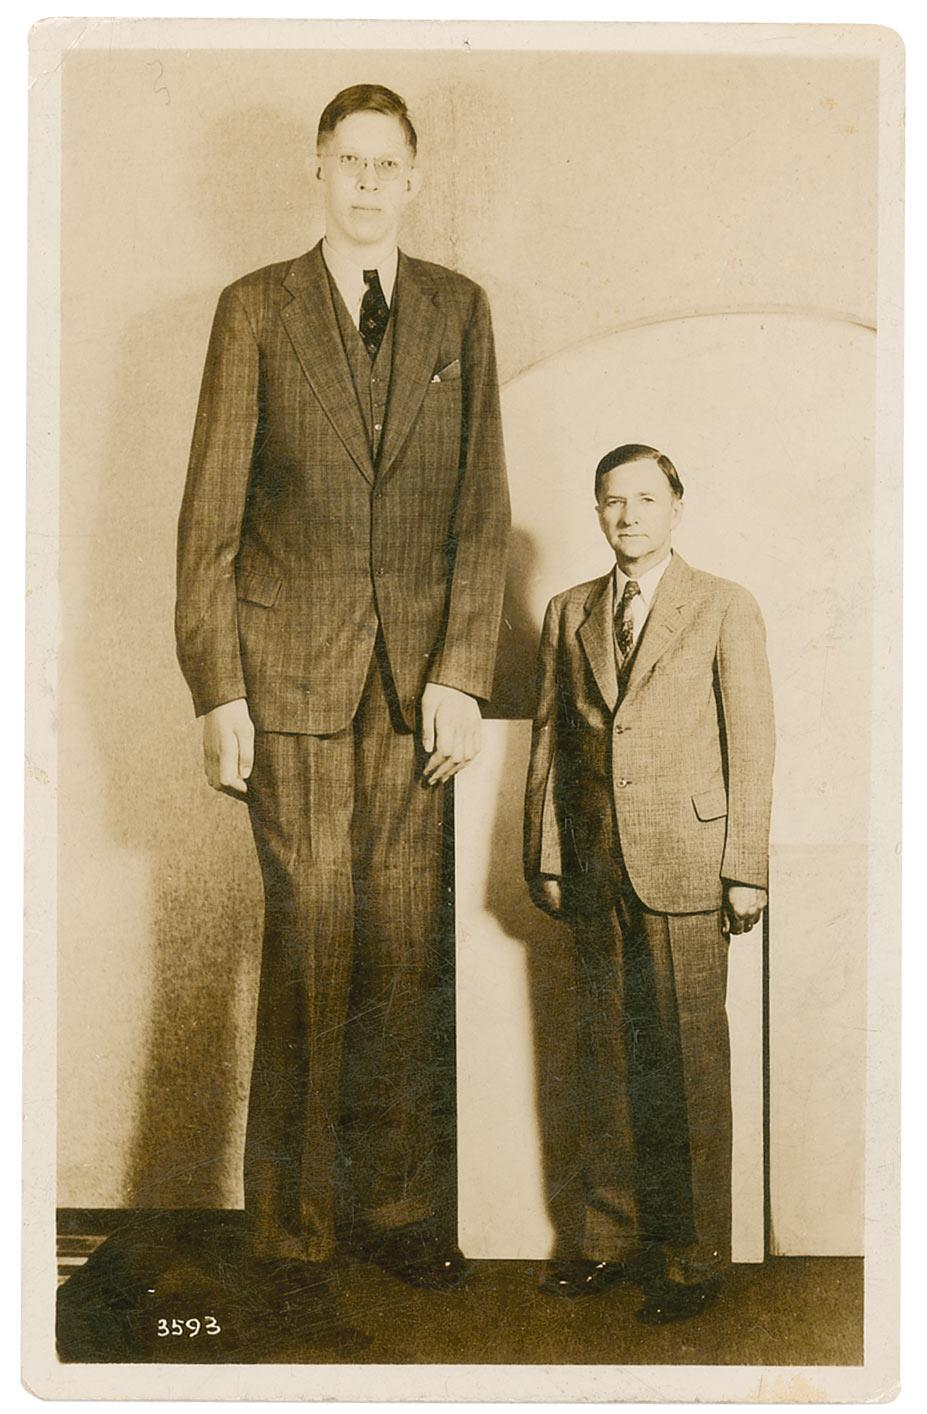
\includegraphics[height=0.5\textheight]{Robert_Wadlow_postcard.jpg}
\caption{A real life giant! Robert Wadlow (left) came in at 8'11" (\(+1\)~SM is 9'). PC: Public Domain (taken from Wikipedia)}
\end{figure}

\chapter{Story}
\begin{commentbox}
\begin{itemize}
\item Where do I want the story to go?
\item What do I want the lynchpin to be?
\end{itemize}
\end{commentbox}

\chapter{Research}
\section{YouTube video: History of Somerset Part 1--}
\begin{itemize}
\item In 1974 when Somerset was broken up (TODO research), it had existed for longer than England itself (\(>1000\)~years!)
\item Buried treasure 3000~years~ago
\item Romans made the first art that tells an entire story (that we have) in Somerset \url{https://museumofsomerset.org.uk/highlights/low-ham-mosaic/} (Could be where the legend of the giants comes from?)
\item 9000 Roman coins found!
\item A \emph{lot} of Roman stuff found around here
\item (Romans left in 410 \textsc{a.d.} and then the dark ages started)
\item Saxons are the ones that have given the Somerset closest to what we know now
\item Quite a few interesting stories about the Celtic missionaries that went to convert people to Christianity. (inc. man that continued to preach when his head had been chopped off!)
\item arguably the smallest parish church in england in somerset
\item \url{https://commons.wikimedia.org/wiki/File:Glastonbury_Abbey_church_from_SW.jpg} became the largest monastic church? in England
\item Somerset had 700 separate estates 
\item Somerset can be called the `Cradle of England' because the king of Wessex made his stand there or something
\item Somerset towns are often fortified because the king of Wessex was a little worried about invasion again
\item Villages started forming around this time, before that it was little settlements
\item All the names of villages are Anglo-saxon
\item Farmers had their pockets filled with gold because of the richness of their land - Thomas Gerard c.~1630
\item Cheddar palace \verb|https://en.wikipedia.org/wiki/Cheddar_Palace|
\item Dragon of Wessex is on a flag
\item Normans built lots of castles
\item crazy continuity exists in Somerset with regards to families
\item 10~C created villages
\item 12~C creates towns
\item Churches would've seemed very large to people living in Somerset
\item First 100\% gothic cathedral -- Wells cathedral 
\end{itemize}


\end{document}
